\epigraph{The difference between ideas and reality is the
difference between philosophy and engineering. The work to transform one into
the other is scientific research}{{\itshape V-Research}}
\begin{figure}[t]
	\centering
	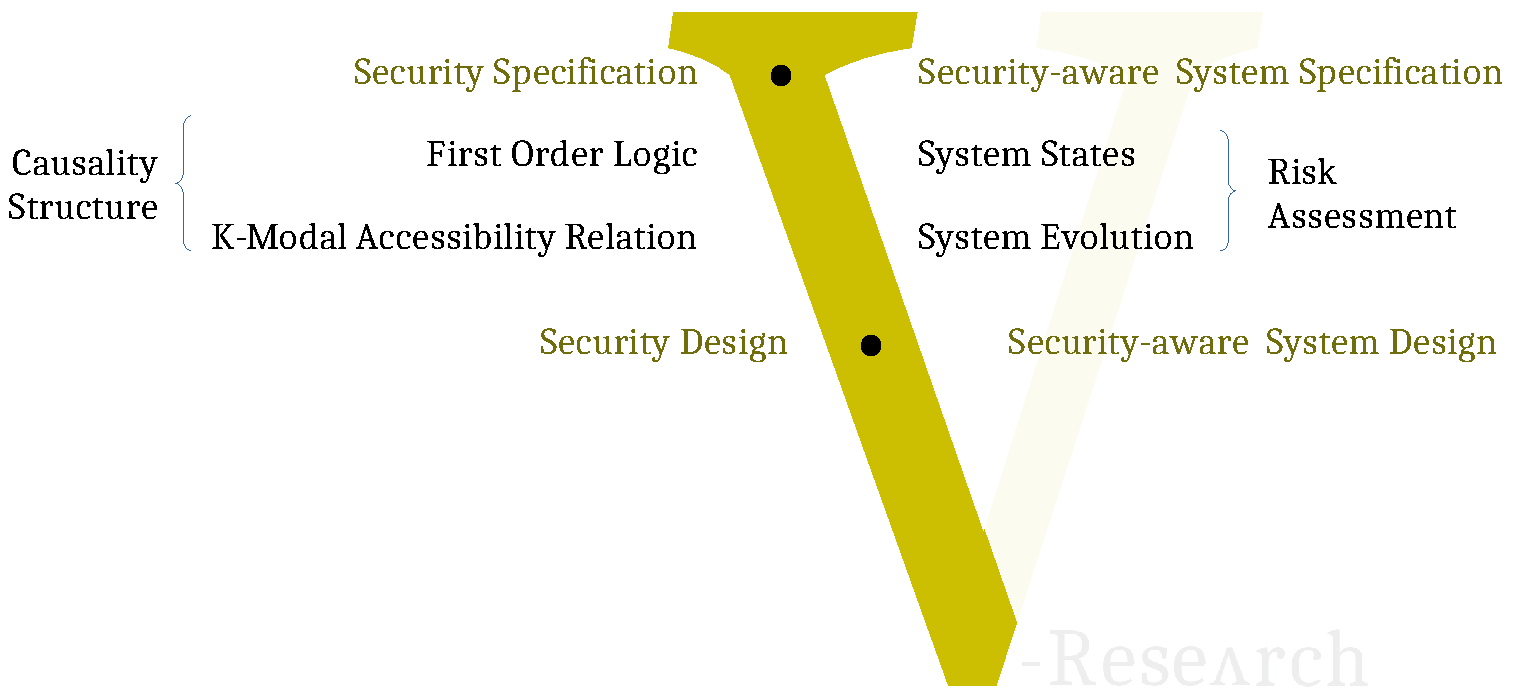
\includegraphics[width=\textwidth]{vmodel.pdf}
	\caption{Cybersecurity Engineering Life-cycle}
	\label{fig:knowledge-belief}
\end{figure}

Infosec, or Information Security, aims at mitigating the security risks related
to information. The standard de-facto is the so called CIA triad 
(where CIA stands for Confidentiality, Integrity, Availability), which is often
criticized for being too general or non-adequate (e.g. by adding authenticity which is 
often used as a building block for confidentiality and integrity) 
to be effectively applied to the engineering of systems. Due to this,
many researchers an organization tried to improve the CIA triad. 
The evolutions/extensions of the CIA triad has been documented, e.g.,
in \autocite{Samonas2014cia} and is summarized in Table~\ref{tab:ciaevolution}.

\begin{table}[h]
\centering
%\setlength{\tabcolsep}{3.5pt}
%\renewcommand{\arraystretch}{1}
\small
\begin{tabular}{rll} 
	{\bf Year} & {\bf Definition} & {\bf Legend}\\
	\hline
	1970s & infosec = CIA & Confidentiality, Integrity, Availability\\
	1980s & infosec += (Au, nR) & Authenticity and non-Repudiation\\
	1990s & infosec += CSpec & Correctness in Specification\\
	2000s & infosec += RITE & Responsibility, Integrity of people, Trust, Ethicality
\end{tabular}
\caption{Chronological progression of the CIA triad~\label{tab:ciaevolution}}
\end{table}


An example is the effort made by the OECD (Organisation for Economic
Co-operation and Development) in \autocite{OECD2013guidelines} to define
security guidelines for information system (1992) based on new principles such
as ``awareness, ethics, risk assessment'' and maintain those revising the
document (e.g.  following the multistakeholder expert consultation in 2013).
Other similar efforts focused on defining entirely new principles or extending
the CIA triad, such as \autocite{NISTSP800-160}. What is of interest for our
argument is that, to the best of our knowledge, all of the approaches that aim
at improving the CIA triad motivated by empirical evidences. On the contrary,
we now define (in Section~\ref{sec:properties}) the CIA triad for an agent
defined in the $\abftheory$ theory and we test if (i) other properties are
allowed in the $\abftheory$ theory, and (ii) if and how the CIA triad can be
detailed in the $\abftheory$ theory.

\subsection{Elicitation of Security Requirements}\label{sec:properties}
In \autocite{Anderson1972report,Samonas2014cia}, CIA are defined as follows.
\begin{itemize}
	\item Unauthorized information release: an unauthorized person is able
		to read and take  advantage  of  information  stored  in  the
		computer.  This  category of concern  sometimes  extends  to
		``traffic  analysis,''  in  which  the intruder  only observes
		the  patterns  of  information  use.  From  those patterns,
		the  intruder can   infer   some   information   content.
		This category   also   includes   the unauthorized use of a
		proprietary program.  (Confidentiality or Secrecy) 
	\item Unauthorized  information  modification:  an  unauthorized person
		is  able  to make changes in stored information -- a form  of
		sabotage.  It should be noted that in the case of this kind of
		violation, the intruder does not necessarily see the
		information he has changed.  (Integrity)
	\item Unauthorized  denial  of  use:  an  intruder  can  prevent  an
		authorized  user  from referring to, or from modifying
		information, even though the intruder may not be able to refer
		to, neither modify the information themselves. (Availability)
\end{itemize}

We now want to generalize the CIA triad to agents and not just 
information and map it to the $\abftheory$ theory.
\begin{definition}{\bf Infosec-Confidentiality --}\label{def:infosec-c}
	An Information $\varphi$ is considered to be confidential to a set of 
	agents $Ag_c$ if, per each agent $a\in Ag_c$, the content of the
	information (i.e. the data it carries) can only be understood (i.e. the relation
	between the information and its data can be known) by the
	agents in $Ag_c$.

	\begin{itemize}
		\item[$(\interpretation21)$] for all agents $a\in Ag$,
			$\world\models\information{a}{\varphi}$ and
			$\world\models\rcc(\varphi,Conf) \wedge
			\neg\dr{Conf}{\varphi}$ iff for any world $\world'$
			such that $\world \modalrelation\world'$,
			$\world'\models\believe{a}{\varphi}$, and
			$\world'\models\knows{a}{\exists f.~
			f(\information{a}{\varphi})=\varphi}$, where 
			$Conf$ is a Region and $f$ is an uninterpreted function.
	\end{itemize}
\end{definition}

\begin{example}{Dummy security protocol --}
	The last part (part III) of the protocol in our first example
	(Figure~\ref{fig:protocol-example}) represents the actual key exchange
	which, in general, needs to be confidential; otherwise the key would be
	known by any other agent who can, e.g., read on the communication
	channel.  Therefore, the last message, in Alice-and-Bob notation can be
	rephrased as: \begin{displaymath} Alice\Rightarrow Bob: enc(pk(Bob),
	symmetricKey) \end{displaymath} where $enc$ is the standard asymmetric
	encryption operator that encrypts the message $symmetricKey$ with the
	public key of Bob $pk(Bob)$ (see, e.g.,
	\autocite{Rocchetto2017interpolation} for a detailed formalization).
	The function $f$ in Definition~\ref{def:infosec-c}, represents any
	function used to enforce confidentiality on information.  In this
	example, $f$ is identified with $enc$ (i.e.
	$enc(pvt(Bob),symmetricKey)=symmetricKey$), the information is
	$\information{Alice}{[enc(pk(Bob),symmetricKey)]}$ and the data, i.e.
	$\varphi$ in Definition~\ref{def:infosec-c}, is $\varphi=symmetricKey$.
	In the perfect cryptography assumption, and assuming for simplicity
	that the logic of the whole protocol preserves confidentiality, the
	message is confidential. In fact, if $Ag={Alice, Bob}$ and $\eq{symmetricKey}{Conf}$:
	\begin{align*}
		\world^0\models\belief{Alice}{symmetricKey},\\
		\world^1\models\information{Alice}{symmetricKey}, \text{and}\\
		\world^2\models\belief{Bob}{symmetricKey} ~\text{if} \\
		enc(pvt(Bob), \information{Alice}{symmetricKey}=symmetricKey)=symmetricKey\\
		(i.e. f=enc ~\text{and}~ \information{Alice}{symmetricKey}=enc(pub(Bob),symmetricKey))\\
	\end{align*}
\end{example}

\begin{definition}{\bf Agent-Confidentiality --}\label{def:confidentiality}
An agent preserves the property of confidentiality iff 
\end{definition}

\begin{definition}{\bf System-Confidentiality --}\label{def:confidentiality}
	The property of confidentiality holds in a system when its information
	preserves confidentiality.
\end{definition}


\fix{mr}{
Confidentiality: the information is accessible only to authorised individuals.
A set of rules that limits access to information.  The information can be
accessed by X if and only if X is authorized to access it = X has the right
attributes (i.e. keys, password) to access it.

Integrity: the information is trustworthy and accurate (i.e. uncorrupted and
unaltered). Protects data from modification or deletion by unauthorized sources
and the ability to undo any damage done.  (for data at rest) If the information
X is written, A will always be read. If information X is modified to
information X', information X can always be recovered.  (for data in transit)
If the information X is sent, A will be received. If information X is modified
to information X', information X can always be recovered.

Availability: the information is accessible and usable when required. Guarantee
of reliable access to the information by authorized people If the information X
needs to be accessed, information X can be retrieved. If

Authenticity: assurance that the information is from the source it claims to be
from. Authenticity involves proof of identity. Authenticity is verified through
authentication.  If information X arrives from A to B, A sent information X and
B can verify it.  ??Authenticity implies integrity but Integrity doesn't imply
authenticity??  ??Authenticity doesn't imply confidentiality but
confidentiality does imply authenticity??

Non-repudiation: the ability to ensure that a party to a contract or a
communication cannot deny the authenticity of their signature on information
(or the sending of) that they originated.  If information X arrives from A, A
sent it and cannot deny it (partial overlap??).  If sender A sends information
X, it cannot say he didn't do it.  Non-repudiation implies authenticity and
integrity. Authenticity doesn't imply non-repudiation (replay attacks?).
Integrity doesn't imply non-repudiation (replay attacks?). 
}

\subsubsection{Relevant Standards}\label{sec:standards}
\begin{enumerate}[noitemsep]
	\item DO-326A
\end{enumerate}

\begin{enumerate}
\item specification -- definition of the desired design of a system. The
specification is verified w.r.t. the  $\abf$ theory. Checking the
controls of the whole cybersecurity life-cycle and the relation with
CWE.
\item design -- the mitigations identified in the specification stage
are implemented into the design. The security of the assets w.r.t. the design are
verified with a, so called, cybersecurity risk assessment.
\end{enumerate}
